\chapter{Behaviour trees}
\label{chap:behaviourtrees}
\section{What Are Behaviour Trees}
\label{sec:behaviourtrees_whatarebehaviourtrees}

Behaviour trees (BTs) are often used in game development to create the behaviour of autonomous agents. They are used to switch between a finite set of tasks and are very modular, making it easy to iterate through different examples. BTs have become popular because they are very good at creating complex behaviours from simple individual tasks. A BT needs different types of nodes to work. \cite{BehaviourTrees}

Depending on the implementation, this may vary slightly, but in general there are four types:

\begin{tabular}{ll}
Composite: & Defines the base rule for how the branch is executed. \cr
Decorator: & Able to modify the return value of a node. \cr
Action: & Contains the logic to be executed when it's invoked. \cr
Conditional: & Used to make Boolean decisions based on the defined condition.
\end{tabular}

Composite nodes are responsible for deciding which action node to call and execute next. It's decision is based on the return value of its children. A node can return the status Running, Success or Failure.

\begin{figure}[H]
	\centering
		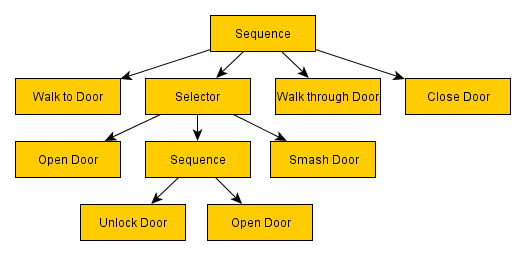
\includegraphics[scale=0.5]{images/behvaiour_tree_example_door.png}
	\caption{Example of a behaviour tree \cite{BehaviourTrees}}
	\label{fig:behvaiour_tree_example_door}
\end{figure}

This is an example of an agent trying to go through a door and then close it. The tree is executed from top to bottom and from left to right. The first node in this example is a composite node, the "Sequence". It starts by executing the leftmost child node and waits for it to finish, in other words, it waits for the "Walk to Door" action to return either success or failure. The Sequence composition works much like an AND operation. It must have all its children return Success for it to also return Success. If only one child returns Failure, it will immediately return Failure. After the first child returns Success, in this example the "Walk to Door" action, it will sequentially execute the next task, which would be the "Selector" node.

The Selector is the opposite of the Sequence node and works like an OR operation. This means that if the first child returns Success, it will also return Success, otherwise it will return Failure. Once the "Selector" node is executed, the agent tries to open the door, and if this fails, the next node is executed, which is another Sequence node. In this sub-tree, the agent will try to unlock the door first and then open it, and if either of these fails, the Smash Door action will be called.

After the door has been opened - by whatever means - the agent will then walk through the door and finally close it. This example consists only of composite and action nodes.

An action node defines the logic that happens when the node is executed. There are also other types of nodes, such as the parallel composite, which allows the actions to be executed in parallel.

Decorators can be used, for example, to invert the return value of an action, or to make it repeat until it returns success or failure.

\section{Example Implementations}
\label{sec:projectevolution_exampleimplementations}

To learn more about behaviour trees, some sample scenes have been created using Unity. For this example, the Behaviour Designer asset from the Unity Asset Store was used, which provides a very intuitive implementation of a behaviour tree.

\subsection{Agent Scene From Advanced 3D Applications}
\label{subsec:projectevolution_exampleimplementations_agentscenefromadvanced3dapplications}

\begin{figure}[H]
    \centering
    \begin{minipage}{0.49\textwidth}
        \centering
        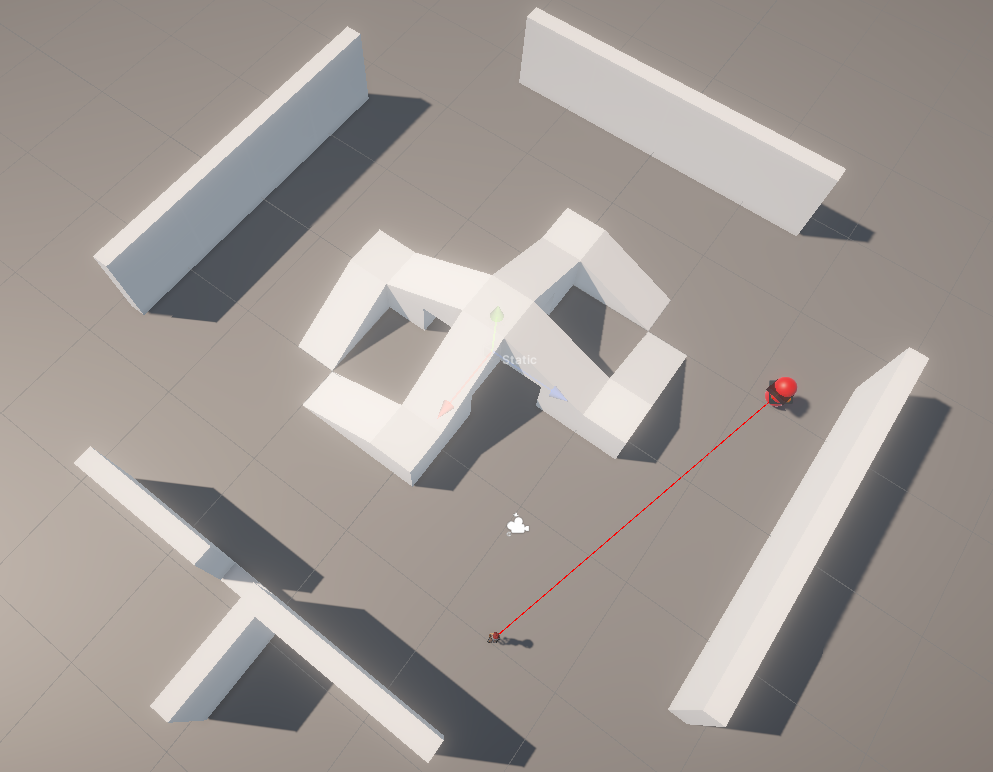
\includegraphics[scale=0.3]{images/behaviour_tree_scene_agent.png}
        \caption{Scene in Unity with the agent}
        \label{fig:behaviour_tree_scene_agent}
    \end{minipage}
    \begin{minipage}{0.49\textwidth}
        \centering
        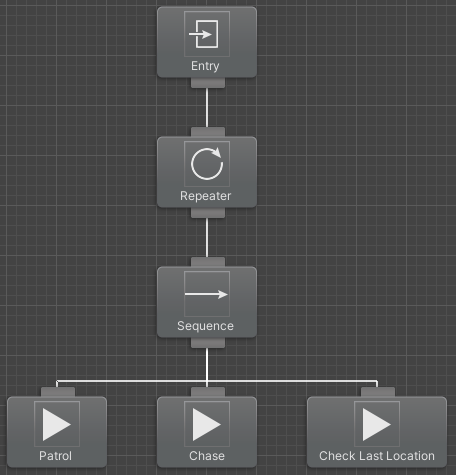
\includegraphics[scale=0.49]{images/behaviour_tree_agent.png}
        \caption{Behaviour tree for the agent}
        \label{fig:behaviour_tree_agent}
    \end{minipage}
\end{figure}


The first example shows an agent who chases the player, called Sintel, as soon as it sees her. The agent will simply patrol the area around him until he sees her, and then start chasing her. Once the line of sight is broken, the agent will check her last location and then resume patrolling.

The BT for this example looks very simple, there is just a repeater node at the top, which will act as an endless loop for the agent. The following Sequence node will therefore continue to execute the three Action nodes from left to right until one of them fails, at which point it will restart with the "Patrol" state.

\subsection{Tour Guide}
\label{subsec:projectevolution_exampleimplementations_tourguide}

\begin{figure}[H]
	\centering
		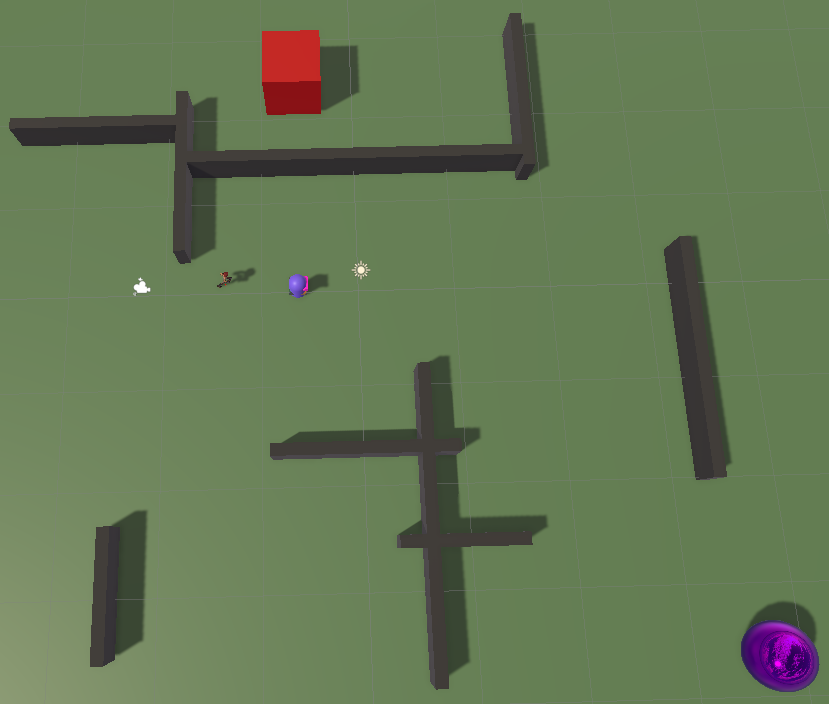
\includegraphics[scale=0.35]{images/behaviour_tree_scene_tour_guide.png}
	\caption{Scene in Unity with the tour guide}
	\label{fig:behaviour_tree_scene_tour_guide}
\end{figure}

As the original idea was to make a tool for a tour guide, the second example shows a tour guide implementation using a BT. The sphere and the cube are placeholders for an object that the tour guide can show to the visitor. The tour guide will first walk to the sphere, say some text there, then walk to the cube while also talking on the way there, and finally talk about the cube. Whenever the visitor is too far away, he will stop and wait for them.

\begin{figure}[H]
	\centering
		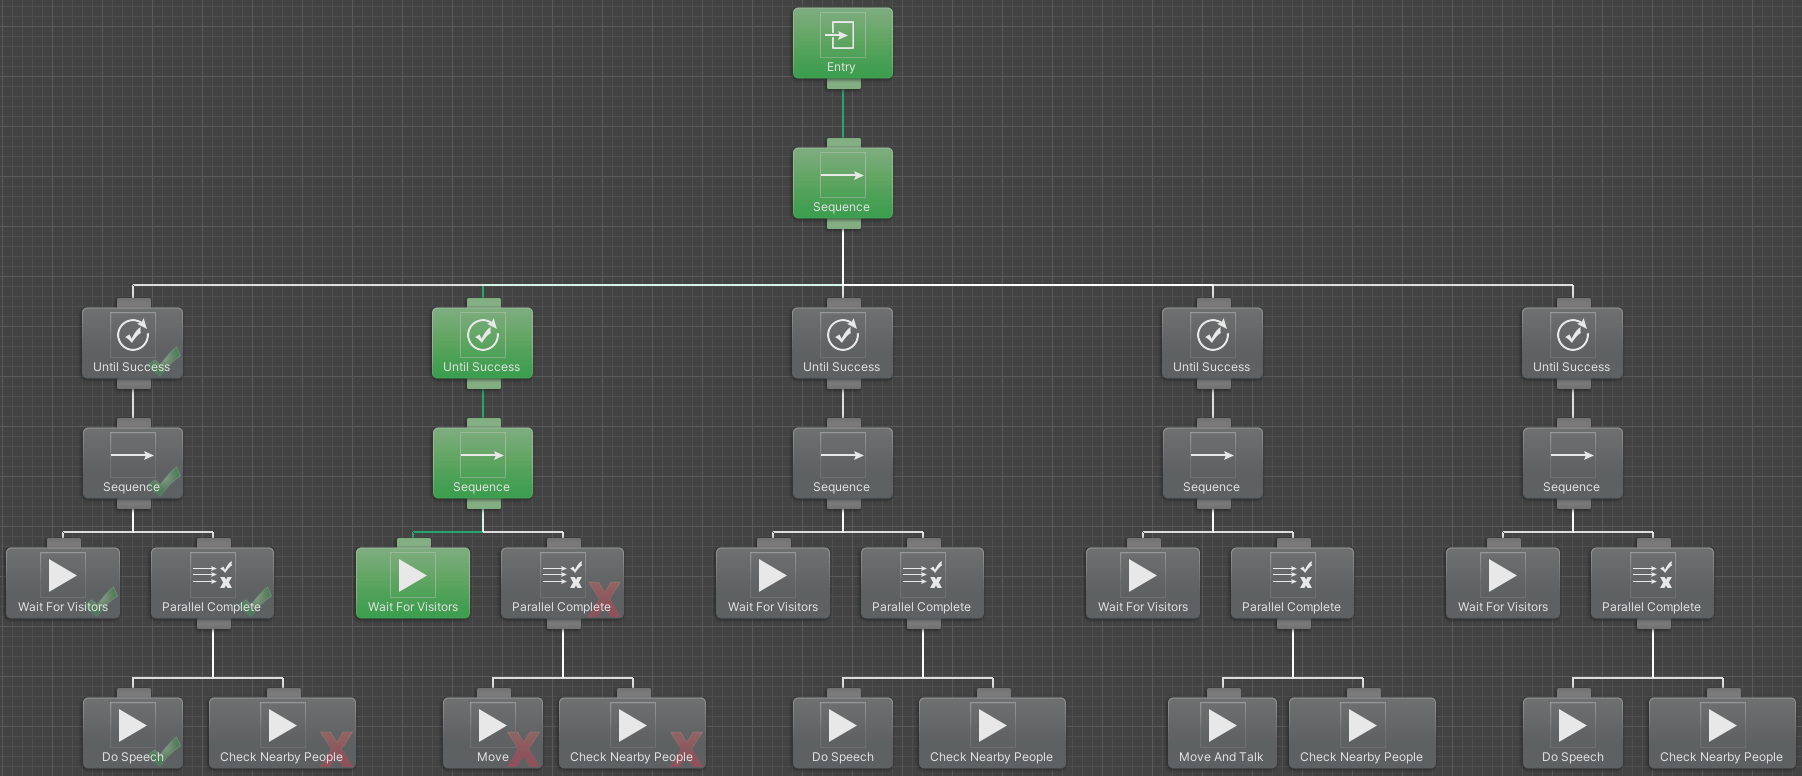
\includegraphics[scale=0.328]{images/behaviour_tree_tour_guide.png}
	\caption{Behaviour tree for the tour guide}
	\label{fig:behaviour_tree_tour_guide}
\end{figure}

This screenshot was taken while the simulation was running, so the current state (in green), the successful states and the failed states of the BT are marked. The first element is a sequence, followed by five subtrees. Each sub-tree is built in the same way: It waits until the visitor is close enough, then does something until the visitor is too far away, at which point it waits again. The bottom left node of each sub-tree tells you what behaviour it will perform.

\section{Strengths}
\label{sec:projectevolution_strengths}

A behaviour tree can be expanded to many hundreds of nodes or even more, and sub-trees can be collapsed for a better overview, making it a very good option for defining simple and complex behaviours.

BTs are also very generic because their action nodes are independent of the overall structure and can be implemented according to the needs of the scenario. Once an action node is implemented, it can be reused over and over again without having to write the same code twice.

In addition to that, BTs are also very intuitive once the basic concept is clear. They can be read and understood by someone who doesn't know much about programming. They're also easy to test and debug, given a good implementation.

\section{Weaknesses}
\label{sec:projectevolution_weaknesses}

Although the behaviour tree is a very powerful concept, it is not perfect for every situation. It starts to have problems when it comes to creating more complex NPCs that can react instantly to any kind of situation, even if some information is missing. BTs are definitely more organised than FSMs and can handle complex behaviour better, but they still suffer from the problem that every possible decision has to be pre-defined manually. Not having to specify the decision for every case would save a lot of time for more intelligent behaviours, and could also make them look more realistic if they were able to decide on their own.

Also, BTs can become expensive as they grow larger, because the cost of evaluation depends heavily on the number of nodes. This is because, naively, the whole tree is evaluated every tick to recompute all the conditions, just to check that the current behaviour is still valid. This can be compensated for by a clever implementation, but it will make the implementation more difficult.
